\documentclass[11pt,a4paper]{article}
\usepackage[utf8]{inputenc}
\usepackage{amsmath}
\usepackage{amsfonts}
\usepackage{amssymb}
\usepackage{graphicx}
\usepackage{booktabs}
\usepackage{multirow}
\usepackage{subcaption}
\usepackage{microtype}
\usepackage{float}
\usepackage[font=footnotesize,labelfont=bf]{caption}
\usepackage[left=2cm,right=2cm,top=2cm,bottom=2cm]{geometry}
\author{Yi Hao}
\title{Dynamics of Heavy-Tailed Initialisation in Deep Learning}
\begin{document}
\maketitle
\begin{abstract}
	While conventional deep learning assumes Gaussian weight statistics, heavy-tailed initialisation ($\alpha < 2$) enable an extended critical regime with superior stability in ordered and chaotic phases. This study investigates the non-equilibrium dynamics of a 10-layer MLP initialised at $\alpha=1.2$ to characterise the transport physics underlying this advantage. We identify a fundamental spatial decoupling: early hidden layers function as a lazy diffusive reservoir, maintaining distributional and geometric stationarity. Conversely, terminal layers exhibit rich learning characterised by ballistic transport kinetics ($\gamma \approx 1.97$) and discrete L\'{e}vy flights that drive staircase performance improvements. Structural analysis reveals that this ballistic state is defined by a $35^\circ$ angular realignment and spectral compression rather than simple mass translation. Furthermore, we observe a dual mechanism of magnitude expansion and tail regularisation, where the network prunes extreme outliers to maintain stability during directed realignment. These results suggest that spatial decoupling and hierarchical division of labour are the primary mechanisms enabling the computational advantages of heavy-tailed architectures.
\end{abstract}
\section{Introduction}
\section{Related Works}
\section{Method}
\subsection{Heavy-Tailed initialisation and Extended Criticality}

To investigate the non-equilibrium dynamics of deep neural networks (DNNs) beyond the Gaussian regime, we initialize the weight matrices $W^l$ using symmetric $\alpha$-stable distributions, as defined by the characteristic function:
\begin{equation} \label{eq:levy_alpha}
    \varphi(u; \alpha, \beta, \sigma, \mu) = \exp\left(-|\sigma u|^\alpha (1 - i\beta \text{sgn}(u)\Phi(u; \alpha)) + iu\mu\right)
\end{equation}
Following the framework of Lévy mean-field theory, we assume a symmetric distribution where the skewness $\beta$ and location $\mu$ are set to zero. The stability parameter (tail index) is set to $\alpha < 2.0$, placing the network within the analytically predicted extended critical regime.

\subsubsection{Scaling Laws and Effective Layer Size}
To ensure consistent signal propagation and avoid the vanishing or exploding gradient problems associated with deep architectures, we adopt a scaling law for the weight entries $W_{ij}^l \sim S_\alpha((D_w / 2N)^{1/\alpha})$. In our implementation, we define an effective width $N_{\text{eff}}$ to normalise the scale parameter across varying layer geometries:
\begin{equation}
    N_{\text{eff}} = 
    \begin{cases} 
      \sqrt{N_{in} \cdot N_{out}} & \text{for linear layers} \\
      C_{in} \cdot K_h \cdot K_w & \text{for convolutional layers}
    \end{cases}
\end{equation}
The scale parameter $\sigma$ for the stable distribution is then computed as:
\begin{equation}
    \sigma = \frac{g}{(2 N_{\text{eff}})^{1/\alpha}}
\end{equation}
where $g$ represents the global gain factor (equivalent to $D_w^{1/\alpha}$ in the manuscript). This normalisation ensures that the fluctuations of the neural input distribution remain stable across the depth of the network. The classical setup is recovered in the $\alpha \rightarrow 2$ limit for comparison with standard Gaussian dynamics.

\subsubsection{Stochastic Implementation}
Weight initialisation is performed using a localised pseudo-random number generator for each layer $l$:
\begin{equation}
    W^l \leftarrow \text{Lévy\_Stable}(\alpha, \beta=0, \sigma, \text{seed} = S_{base} + l)
\end{equation}
By decoupling the random seeds across layers, we prevent the formation of correlated super-paths of outliers through the network depth. This ensures that the observed multifractal properties of the layerwise Jacobians are a result of the collective heavy-tailed dynamics rather than initialisation artifacts.

\subsection{Dynamical Observables: Layer-wise Displacement Tracking}

To quantify the evolution of the network weight manifold during training, we define three primary scalar observables derived from the weight displacement vector. Let $W^l_t$ denote the weight matrix of layer $l$ at training step $t$. For a specific time lag $\tau$, the displacement matrix is defined as $\Delta W^l(t, \tau) = W^l_t - W^l_{t-\tau}$. These metrics allow us to distinguish between stochastic noise, collective drift, and high-energy structural realignments.

\subsubsection{Mean Net Displacement (Drift)}
The Mean Net Displacement, $\mu_{\Delta W}$, represents the collective drift or centre-of-mass movement of the parameters in layer $l$:
\begin{equation}
    \mu_{\Delta W}(t, \tau) = \frac{1}{N_l} \sum_{i,j} \Delta W^l_{ij}(t, \tau)
\end{equation}
where $N_l$ is the total parameter count for the layer. This observable serves as a dynamical indicator of symmetry breaking; values fluctuating near zero suggest a state of local stochastic equilibrium, whereas sustained plateaus signify a directed migration toward a new representation.

\subsubsection{Mean Absolute Displacement (L1 Activity)}
The Mean Absolute Displacement provides a measure of the total integrated activity of the layer, independent of direction:
\begin{equation}
    \mu_{|\Delta W|}(t, \tau) = \frac{1}{N_l} \sum_{i,j} |\Delta W^l_{ij}(t, \tau)|
\end{equation}
This $L_1$ metric captures the typical scale of weight updates. It is used to identify the thermal floor of the training process and detect changes in the overall volume of weight exploration across different network depths.

\subsubsection{Root Mean Square Displacement (L2 Energy)}
The Root Mean Square (RMS) displacement, or $L_2$ norm, characterises the total kinetic energy of the layer-wise updates:
\begin{equation}
    \text{RMS}_{\Delta W}(t, \tau) = \sqrt{\frac{1}{N_l} \sum_{i,j} \left( \Delta W^l_{ij}(t, \tau) \right)^2}
\end{equation}
By squaring the displacements before averaging, the $L_2$ norm is significantly more sensitive to outliers than the $L_1$ norm. In networks initialised with heavy-tailed distributions ($\alpha < 2$), this observable is the primary detector for Lévy flights, discrete, high-magnitude realignments that dominate the transport physics in the extended critical regime.

\subsubsection{Multi-Scale Temporal Analysis}
To separate microscopic noise from macroscopic learning, these metrics are tracked across two distinct time lag regimes:
\begin{enumerate}
    \item \textbf{Microscopic Lag ($\tau < 1$ epoch):} Captures the instantaneous stochastic gradient noise and the thermal floor of the initialisation.
    \item \textbf{Macroscopic Lag ($\tau \geq 1$ epoch):} Acts as a low-pass filter to reveal persistent structural drift and global phase transitions that are otherwise obscured by step-wise jitter.
\end{enumerate}

All macroscopic lag data points are timestamped at the window midpoint, $t - \tau/2$, to ensure causal alignment between internal weight reorganisation and external performance metrics such as test accuracy and loss.

\subsection{Transport Kinetics and TAMSD Estimators}
To characterise the diffusion regimes, we employ the Time-Averaged Mean Squared Displacement (TAMSD), defined for a trajectory $x(t)$ of length $T$ and time lag $\tau$ as:
\begin{equation}
	\langle \delta^2(\tau) \rangle = \frac{1}{T-\tau} \int_0^{T-\tau} [x(t+\tau) - x(t)]^2 dt
\end{equation}
The diffusion exponent $\gamma$ is extracted via a local power-law fit $\langle \delta^2(\tau) \rangle \propto \tau^\gamma$. We utilise a sliding-window regression to monitor the non-stationarity of $\gamma$ throughout the training trajectory.
\subsection{Structural and Spectral Observables}
To monitor the emergence of low-rank manifolds and feature specialisation, we track the singular value spectrum $\{\lambda_i\}$ of the weight matrices.

\subsubsection{Spectral Gap and Compression}
The spectral gap is defined as the ratio of the two most dominant singular values, $\Gamma = \lambda_1 / \lambda_2$. An increase in $\Gamma$ signifies the emergence of a dominant feature direction. Concurrently, we track the stable rank $\mathcal{R}_s = \|W\|_F^2 / \|W\|_2^2$, which provides a continuous measure of the matrix's effective dimensionality.

\subsubsection{Angular Realignment}
To decouple weight growth from feature rotation, we utilise the layer-wise cosine distance:
\begin{equation}
	d_{cos}(W_t, W_0) = 1 - \frac{\text{Tr}(W_t^\top W_0)}{\|W_t\|_F \|W_0\|_F}
\end{equation}
This metric quantifies the geometric rotation of the weight vector in the high-dimensional parameter space, independent of changes in the Frobenius norm.
\subsection{Distributional Heavy-Tail Analysis}
We utilize the Complementary Cumulative Distribution Function (CCDF) to analyze the tail behavior of weight magnitudes $|W|$. The CCDF is defined as $P(|W| > x) = 1 - F(x)$, where $F(x)$ is the cumulative distribution function. To monitor the stability of the heavy-tailed initialization, we periodically estimate the tail index $\alpha$ using the McCulloch quantile-based method, which provides a robust fit for $\alpha$-stable distributions.
\subsection{Inter-layer Dynamical Correlations}
To identify collective layer-wise behaviors, we compute the correlation matrices of $L_2$ displacements across all network layers. We employ three distinct metrics: (i) Pearson correlation for linear dependencies, (ii) Spearman’s rank correlation for monotonic non-linear relationships, and (iii) Distance Correlation to capture complex, non-monotonic dependencies between dynamical regimes.
\section{Experiments}
\subsection{Dataset and Preprocessing}
All experiments are conducted using the MNIST dataset of handwritten digits. The input data consists of $28 \times 28$ grayscale images, which are flattened into vectors of size 784. Preprocessing involves a standard normalisation transform with a mean of 0.1307 and a standard deviation of 0.3081. We utilise a consistent batch size of 1024 to maintain stable gradient estimates across all initialisation regimes.

\subsection{Model Architecture}
To study the impact of heavy-tailed statistics on non-equilibrium learning dynamics, we employ a deep Multilayer Perceptron (MLP) consisting of $L=10$ layers (9 hidden layers and one output classifier). The network maps an input vector $x^0 \in \mathbb{R}^{784}$ to an output $x^L \in \mathbb{R}^{10}$ through a sequence of transformations:
\begin{equation}
    x^l = \phi(W^l x^{l-1} + b^l)
\end{equation}
where $\phi$ is the activation function. The specific architectural constraints are defined as follows:

\begin{itemize}
    \item \textbf{Layer-wise Dimensions:} We maintain a constant hidden width of $N=784$ neurons for all layers $l \in \{1, \dots, L-1\}$. This configuration ensures that the weight matrices $W^l$ are square ($N \times N$), facilitating direct comparisons with results from Random Matrix Theory (RMT) and free probability.
    \item \textbf{Weights ($W$):} The weight matrices $W^l$ are initialised according to a symmetric $\alpha$-stable distribution. This initialisation places the network within the extended critical regime, distinct from standard Gaussian ($\alpha=2$) initialisations.
    \item \textbf{Activation ($\phi$):} The hyperbolic tangent ($\tanh$) function is utilised for all hidden layers to ensure bounded signal propagation and centred activations.
    \item \textbf{Biases ($b$):} All bias terms are explicitly disabled ($b^l=0$) to isolate the dynamical effects of the weight matrix couplings and simplify the analysis of the layer-wise Jacobians.
\end{itemize}

\subsection{Heavy-Tailed initialisation Strategy}
The core of this research involves a parametric sweep over non-Gaussian weight initialisation. Weights are sampled from a symmetric L\'{e}vy $\alpha$-stable distribution defined by Eq. \ref{eq:levy_alpha}. We explore a $3 \times 3$ grid of hyperparameters to compare different dynamical phases:
\begin{itemize}
    \item \textbf{Stability Parameter ($\alpha$):} Fixed at $\{1.2, 1.5, 2.0\}$. Here, $\alpha=2.0$ serves as the Gaussian baseline, while $\alpha < 2.0$ introduces heavy-tails with infinite variance.
    \item \textbf{Scale Parameter ($g$):} Fixed at $\{0.25, 1.0, 3.0\}$. This parameter dictates the coupling strength $D_w^{1/\alpha}$, allowing us to move the network through ordered, critical, and chaotic regimes.
\end{itemize}

\subsection{Optimisation and Training Protocol}
The networks are trained for 650 epochs using vanilla Stochastic Gradient Descent (SGD). We set a fixed learning rate of $\eta = 0.001$. Notably, we omit momentum and weight decay; this ensures that any observed structural evolution or rich learning behaviour is a direct result of the interaction between the heavy-tailed initialisation and the fundamental SGD trajectory. All simulations are executed on NVIDIA hardware using the PyTorch framework with a fixed seed ($s=0$) to ensure exact reproducibility across parameter sweeps.
\section{Results}
The performance of the 10-layer MLP was evaluated across a $3 \times 3$ grid of initialisation parameters, varying the tail index $\alpha \in \{1.2,1.5,2.0\}$ and the scale factor $\sigma \in \{0.25,1.0,3.0\}$. These parameters were selected to represent the ordered, critical, and chaotic regimes, respectively.

\begin{figure}[htbp]
    \centering
    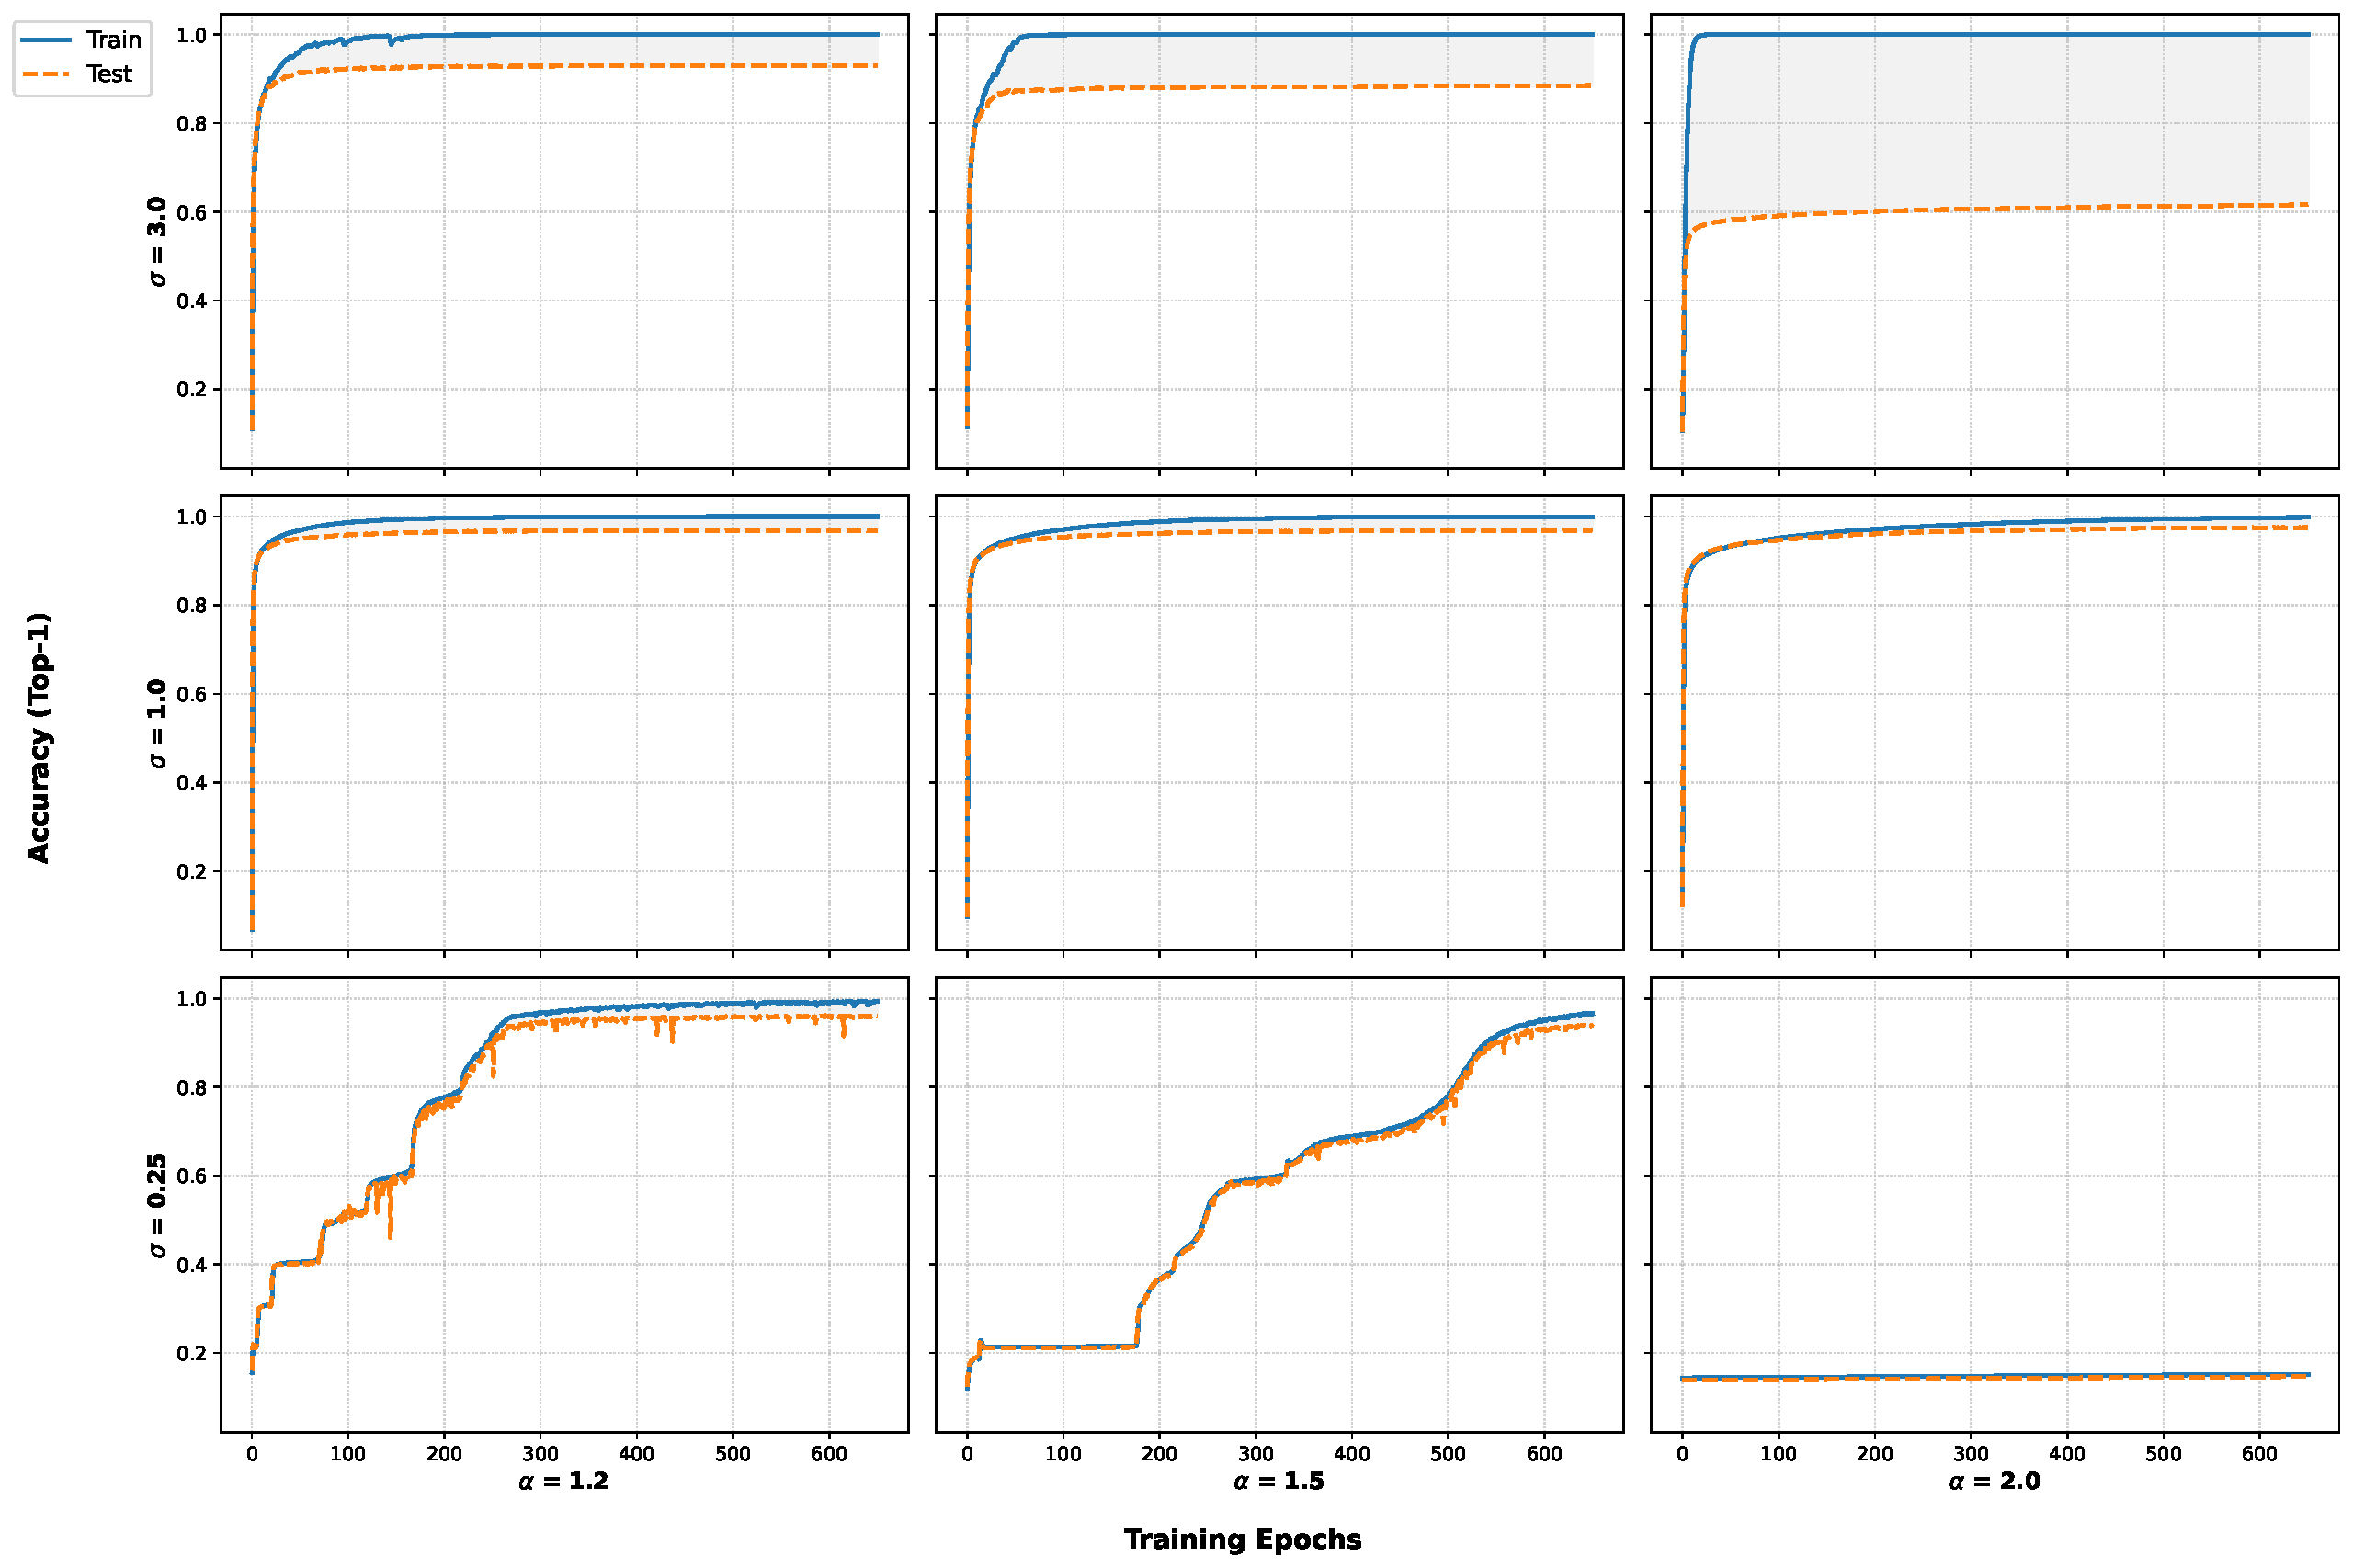
\includegraphics[width=\textwidth]{performance_runs.pdf}
    \caption{Accuracy curves for 10-layer MLP trained on MNIST. Initialisation varies from Gaussian ($\alpha = 2.0$) to strongly heavy-tailed ($\alpha = 1.2$), while the three scale values of $\sigma = 0.25, 1.0, 3.0$ are chosen to represent the ordered, critical, and chaotic regimes respectively. Generalisation gap is highlighted in grey.}
    \label{fig:performance_curves}
\end{figure}

The training profiles across the $3\times3$ parameter sweep, as detailed in Figure \ref{fig:performance_curves} and Table \ref{tab:performance_summary}, exhibit dynamical behaviours consistent with the extended critical regime described in recent theoretical frameworks. 

The training trajectories and final performance metrics, summarised in Table \ref{tab:performance_summary}, reveal distinct behaviours across the parameter space. Within the critical regime ($\sigma=1.0$), all configurations exhibit robust convergence. The Gaussian ($\alpha=2.0$) initialisation achieves the highest test accuracy in this regime at 0.9751, followed closely by the heavy-tailed variants. However, as the system moves into the ordered and chaotic regimes, a significant divergence in performance emerges.

In the chaotic regime ($\sigma=3.0$), the Gaussian network suffers from a substantial generalisation gap of 0.3836. In contrast, the heavy-tailed configurations ($\alpha=1.2,1.5$) demonstrate superior stability, maintaining test accuracies above 85\%, with the $\alpha=1.2$ run achieving 0.9297. This suggests that heavy-tailed initialisation may provide a degree of protection against the informational expansion typically associated with chaotic phases.

\begin{table}[htbp]
\centering
\caption{Final Performance Summary across Initialisation Scales ($\sigma$) and Tail Thickness ($\alpha$).}
\label{tab:performance_summary}
\begin{tabular}{lccccr}
\toprule
\textbf{Scale ($\sigma$)} & \textbf{Tail ($\alpha$)} & \textbf{Train Acc} & \textbf{Test Acc} & \textbf{Gen. Gap ($\Delta$)} \\ \midrule
\multirow{3}{*}{3.00} & 1.2 & 1.0000 & 0.9297 & 0.0703 \\
                      & 1.5 & 1.0000 & 0.8855 & 0.1145\\
                      & 2.0 & 1.0000 & 0.6164 & 0.3836\\ \hline
\multirow{3}{*}{1.00} & 1.2 & 0.9999 & 0.9683 & 0.0316 \\
                      & 1.5 & 0.9998 & 0.9692 & 0.0306 \\
                      & 2.0 & 0.9982 & 0.9751 & 0.0231 \\ \hline
\multirow{3}{*}{0.25} & 1.2 & 0.9932 & 0.9602 & 0.0330 \\
                      & 1.5 & 0.9654 & 0.9365 & 0.0289 \\
                      & 2.0 & 0.1522 & 0.1468 & 0.0054 \\ \bottomrule
\end{tabular}
\end{table}

The ordered regime ($\sigma=0.25$) presents perhaps the most striking dynamical shift. While Gaussian learning appears stagnant, with accuracy remaining near-constant at $\approx$0.15, the heavy-tailed runs exhibit a unique staircase trajectory. These curves are characterised by prolonged plateaus followed by abrupt, high-magnitude increases in accuracy. Such behaviour is suggestive of discrete phase transitions or non-uniform learning bursts, where the network periodically escapes local minima to reach a higher performance state.

Given the highly differentiated dynamics observed in the ordered regime, the remainder of this analysis will focus on the ($\alpha=1.2,\sigma=0.25$) configuration. This case offers a unique opportunity to investigate the internal weight displacements and structural reorganisation events that characterise heavy-tailed learning in traditionally silent regimes.
\subsection{Spatial Decoupling in Layer-wise Dynamics}
\begin{figure}[htbp]
    \centering
    \begin{subfigure}{0.48\textwidth}
        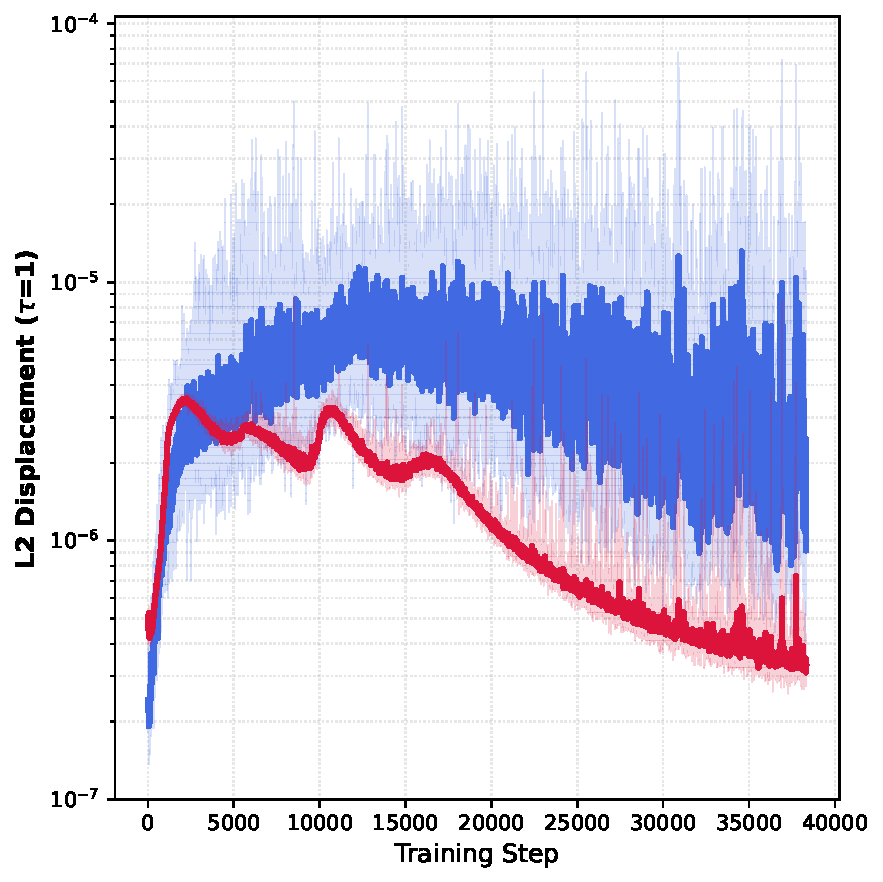
\includegraphics[width=\textwidth]{layer_dynamics_fast.pdf}
        % \caption{Micro-scale kinetics ($\tau=1$)}
        \phantomcaption
        \label{fig:dyn_micro}
    \end{subfigure}
    \begin{subfigure}{0.48\textwidth}
        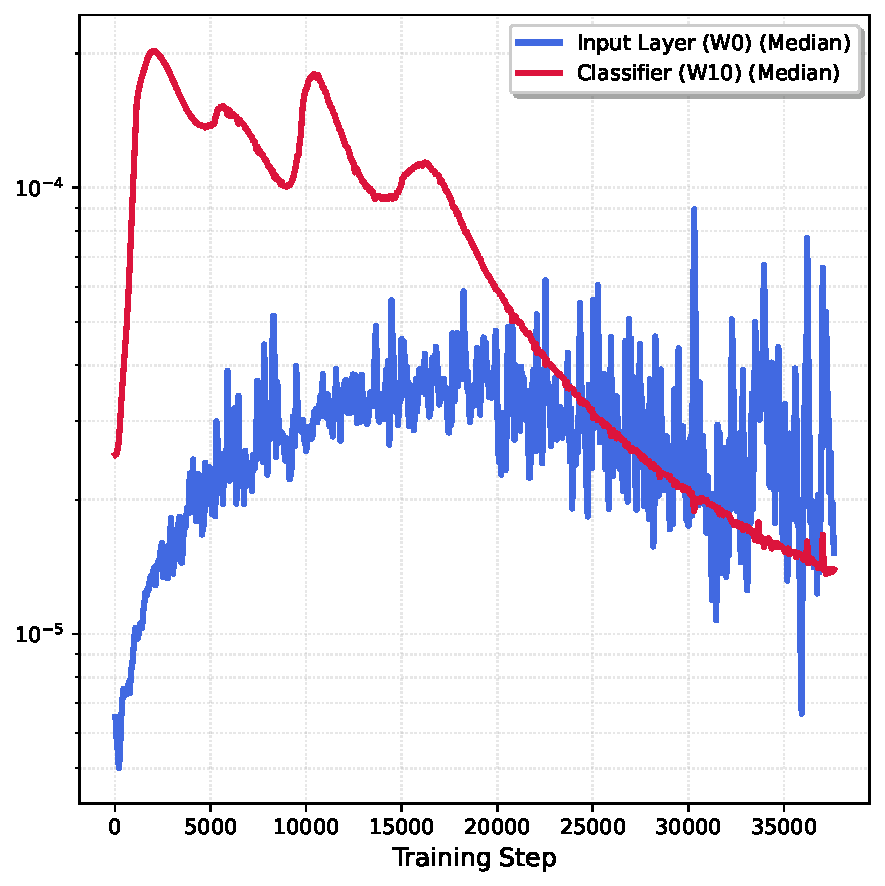
\includegraphics[width=\textwidth]{layer_dynamics_slow.pdf}
        % \caption{Macro-scale kinetics ($\tau=58$)}
        \phantomcaption
        \label{fig:dyn_macro}
    \end{subfigure}
    \vspace*{-2em}
    \caption{Temporal evolution of $L_2$ weight displacement. (a) Step-wise dynamics ($\tau=1$) showing raw fluctuations and a 15-step rolling median. (b) Epoch-wise displacement ($\tau=58$) highlighting the contrast in trajectory smoothness between layers.}
    \label{fig:dynamics}
\end{figure}
\newpage
The layer-wise kinetics displayed in Figure \ref{fig:dynamics} reveal a distinct divergence in the dynamical evolution of the network. For the input layer ($W^1$), the $L_2$ displacement follows a tri-phasic trajectory: an initial rapid ascent from $10^{-6}$ to $10^{-5}$ within the first 2500 steps, followed by a secondary rise to the upper $10^{-5}$ range, and a final gradual descent. Notably, $W^1$ maintains a high, gradually increasing variance throughout the training process, characterised by persistent stochastic fluctuations at the micro-scale ($\tau=1$).

In contrast, the classifier ($W_{10}$) exhibits a non-monotonic displacement pattern. Following an initial shared ascent with the input layer, $W_{10}$ enters a regime characterised by undulating pulses that persist until approximately step 17,000, after which the displacement follows a steady decay. At the $\tau=1$ scale (Fig. \ref{fig:dyn_micro}), $W_{10}$ is distinguished by a low baseline noise floor punctuated by intermittent, high-magnitude spikes. 

A comparison between the micro-scale and macro-scale ($\tau=58$) kinetics in Figure \ref{fig:dyn_macro} reveals a shift in relative magnitudes. At the $\tau=1$ scale, the displacement of $W_{10}$ is consistently lower than or equal to $W^1$. However, at the $\tau=58$ scale, the magnitude of $W_{10}$ meets or exceeds that of $W^1$. Furthermore, the high-frequency variance observed in $W_{10}$ at the step-scale largely vanishes when viewed at the epoch-scale, resulting in a smooth trajectory. Conversely, the input layer maintains significant oscillatory behaviour across both time lags.

\begin{figure}[htbp]
    \centering
    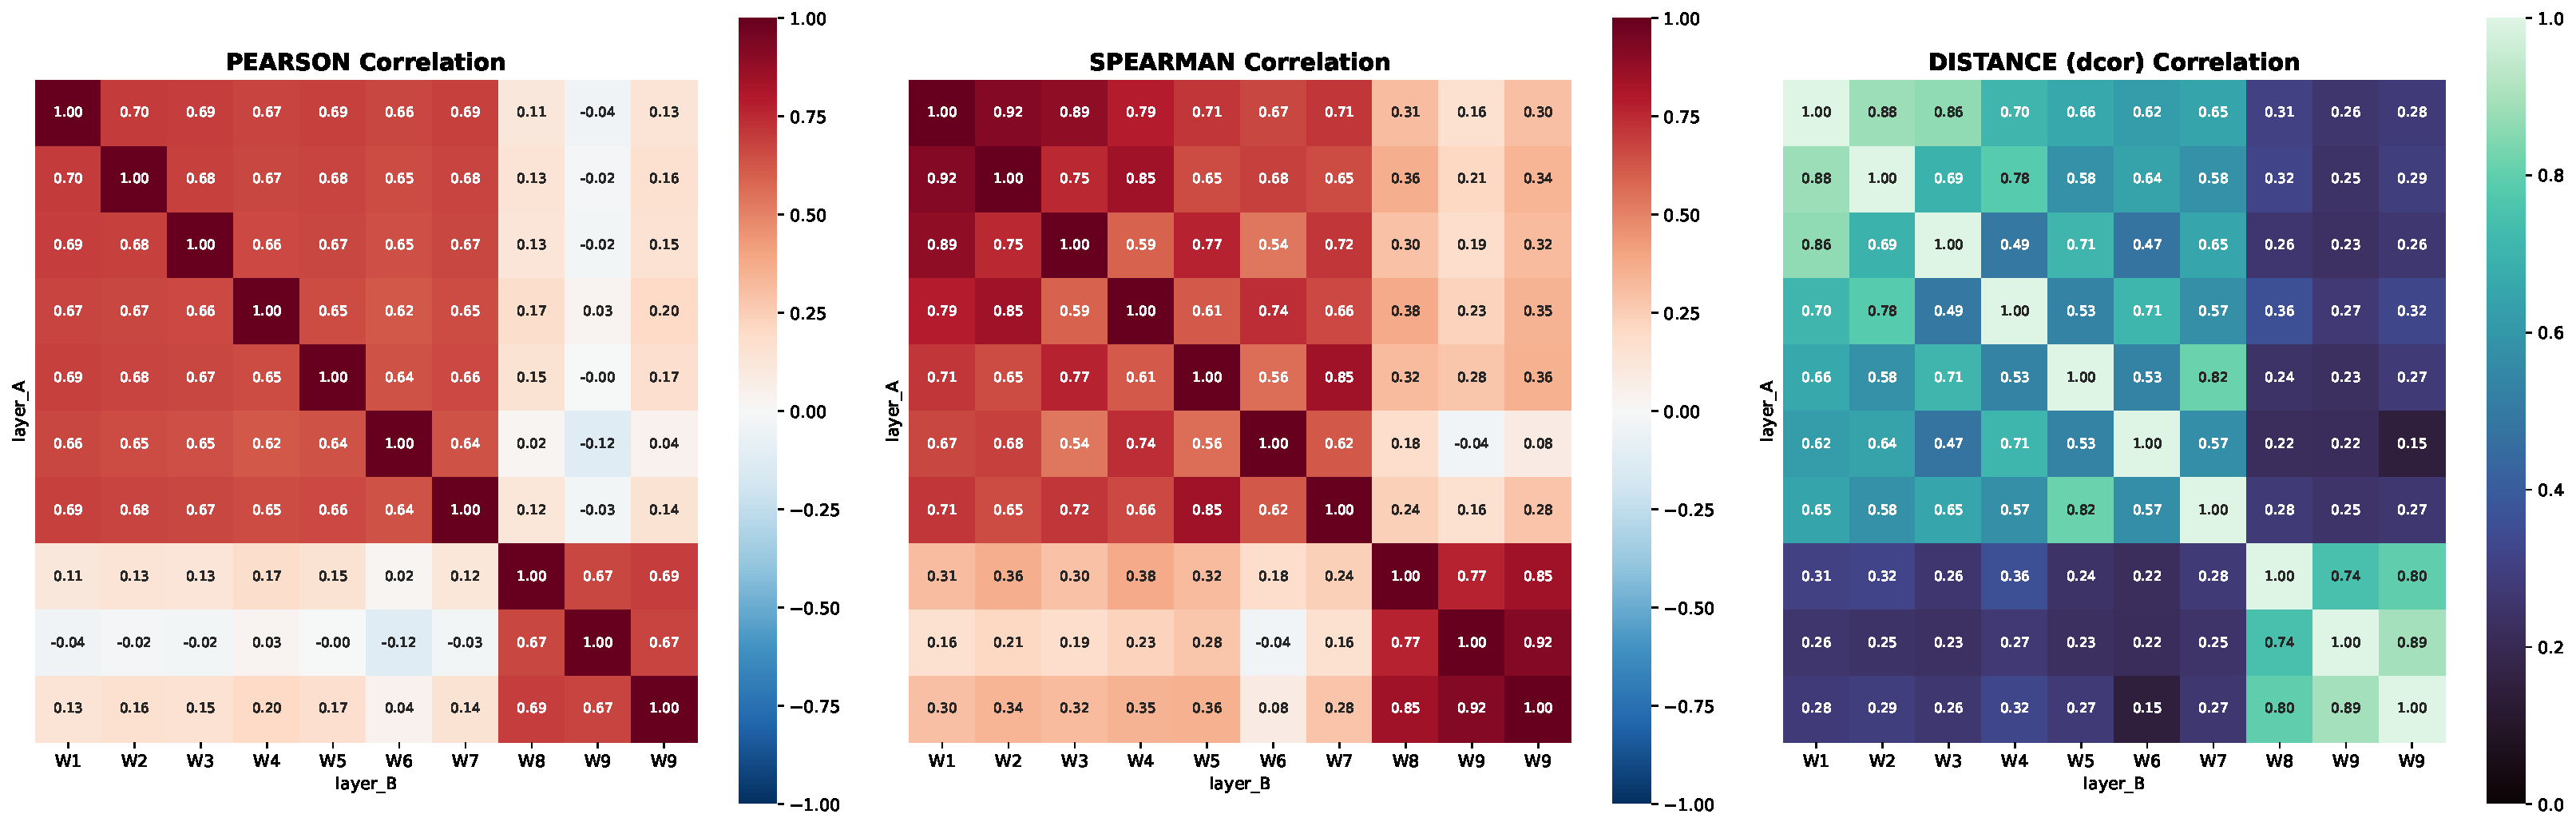
\includegraphics[width=0.9\textwidth]{correlations.pdf}
    \caption{Inter-layer correlation matrices of $L_2$ weight displacements ($\tau=1$). The emergence of block-diagonal structures suggests a partitioning of the network into two dynamically independent regions.}
    \label{fig:correlations}
\end{figure}

The global organisation of these dynamics is further quantified via the correlation matrices in Figure \ref{fig:correlations}. Across Pearson, Spearman, and Distance Correlation metrics, a consistent block-diagonal structure emerges, indicating that the observed dynamics are representative of collective layer behaviours. The network appears to partition into two independent blocks: a primary block spanning layers $W^1$ through $W^7$, and a secondary block comprising $W^8$ through $W_{10}$. 

Within these identified blocks, we observe moderately high correlations (ranging from $0.6$ to $0.7$ for Pearson), while inter-block correlations drop significantly ($< 0.2$ or negative). We further note that while the Pearson matrix indicates relatively uniform coupling within each block, the Spearman and Distance Correlation matrices display a more heterogeneous checkerboard pattern, with localised correlations fluctuating between $0.5$ and $0.9$. This suggests that while linear trends are shared across layers within a block, the underlying non-linear dependencies exhibit a higher degree of local variation.
\newpage
\subsection{Diffusion Regime Identification via TAMSD}

To rigorously categorise the transport physics of the network, we analyse the Time-Averaged Mean Squared Displacement (TAMSD) on a log-log scale. The scaling exponent $\gamma$, defined by $\langle \Delta x^2 \rangle \sim \tau^\gamma$, provides a quantitative measure of the diffusion regime, where $\gamma = 1$ denotes Brownian motion, $\gamma < 1$ signifies sub-diffusion, and $\gamma \approx 2$ indicates ballistic or directed motion.

\begin{figure}[htbp]
    \centering
    \begin{subfigure}{0.48\textwidth}
        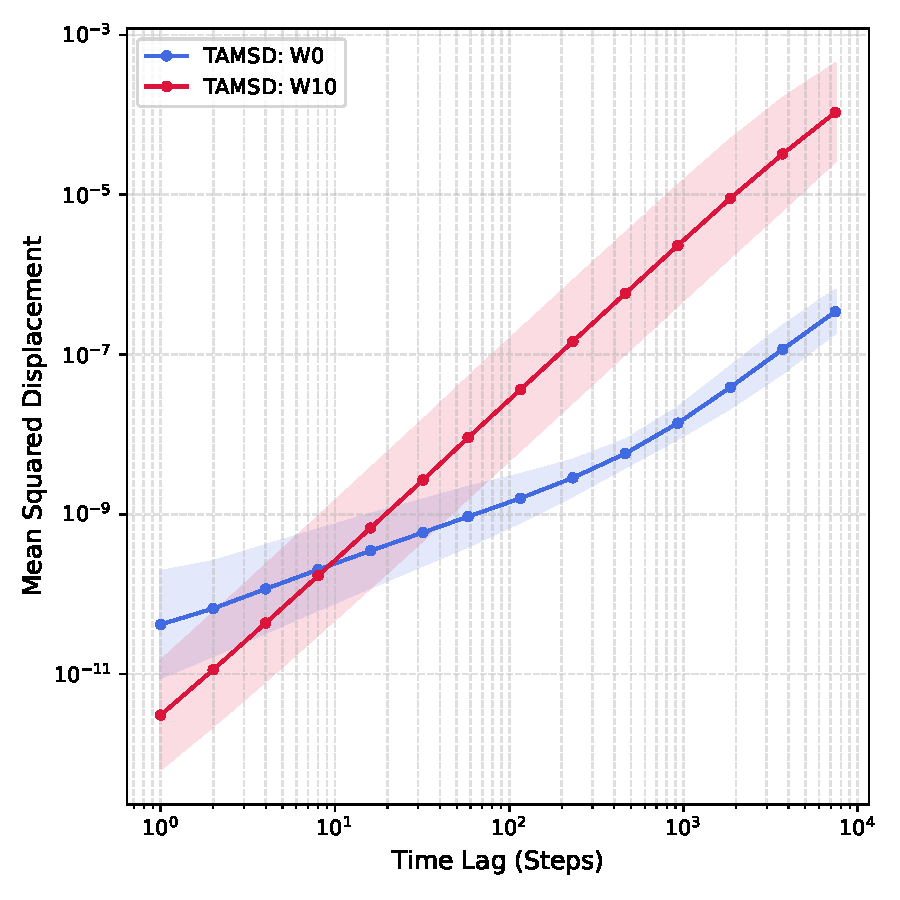
\includegraphics[width=\textwidth]{tamsd_comparison.pdf}
        % \caption{TAMSD Scaling Contrast}
        \phantomcaption
        \label{fig:tamsd_compare}
    \end{subfigure}
    \begin{subfigure}{0.48\textwidth}
        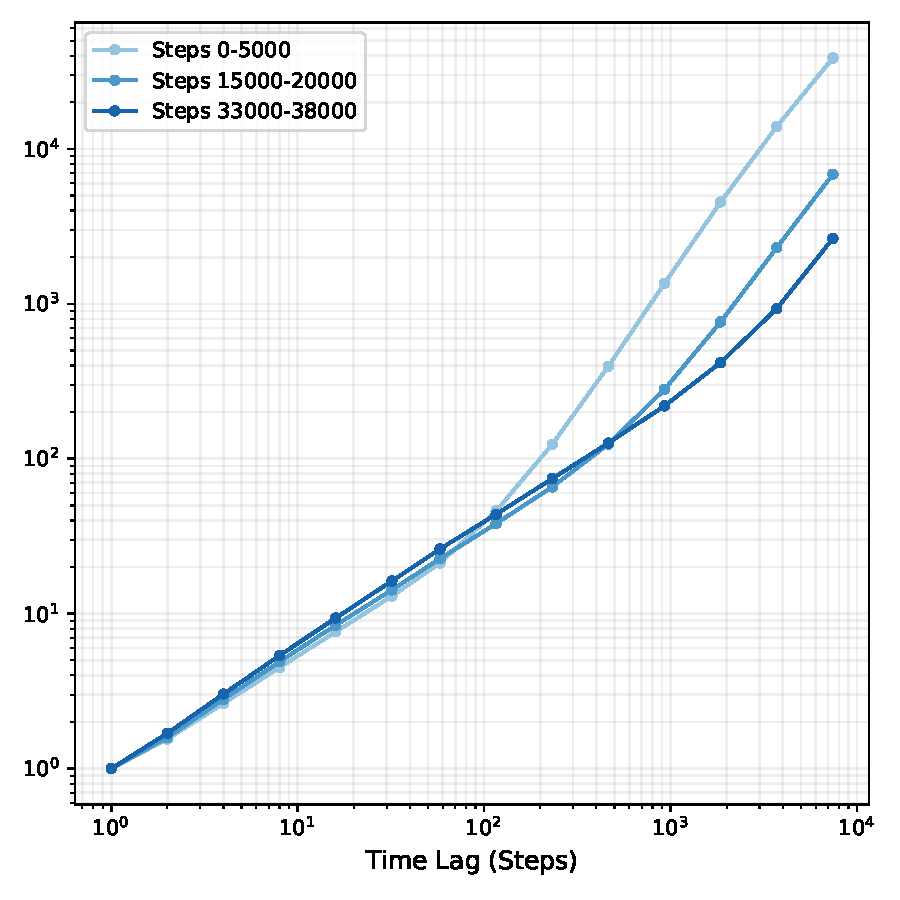
\includegraphics[width=\textwidth]{tamsd_evolution.pdf}
        % \caption{Normalized $W^{0}$ Branching}
        \phantomcaption
        \label{fig:tamsd_evo}
    \end{subfigure}
    \vspace*{-2em}
    \caption{Log-log profiles of the TAMSD. (a) Comparison of the initial layer $W^{0}$ and classifier $W^{10}$, with shaded regions representing the multiplicative standard deviation (geometric SD). (b) Temporal evolution of the normalised TAMSD for $W^{0}$, highlighting the shift in crossover points across training epochs.}
    \label{fig:tamsd}
\end{figure}

As illustrated in Figure \ref{fig:tamsd_compare}, we observe a fundamental bifurcation in transport regimes between the network's extremities. For the classifier ($W^{10}$), the dynamics are characterised by a near-perfect ballistic exponent of $\gamma = 1.974 \pm 0.014$. This suggests a regime dominated by a consistent, high-magnitude gradient signal where stochastic fluctuations are negligible relative to the directional drift. Conversely, the initial layer ($W^{0}$) exhibits anomalous diffusion with a global exponent of $\gamma = 0.968 \pm 0.085$.

The increased uncertainty ($\sigma_\gamma$) for $W^{0}$ is indicative of a non-linear crossover in log-log space. Specifically, $W^{0}$ exhibits a sub-diffusive regime ($\gamma \approx 0.78$) at short time lags ($\tau < 300$) before transitioning to a super-diffusive drift ($\gamma \approx 1.49$) at macro-scale lags. Notably, the geometric standard deviation for $W^{10}$ remains scale-invariant, whereas for $W^{0}$, the variance narrows significantly in the macro-scale regime. This implies that while $W^{0}$ is locally noisy, it converges toward a more stationary and consistent velocity when viewed over larger temporal horizons.

Figure \ref{fig:tamsd_evo} further elucidates the non-stationarity of these dynamics by normalising the TAMSD relative to the unit lag ($\tau=1$). We observe a temporal shift in the crossover point; during early training (Steps 0--5000), the transition to super-diffusion occurs an order of magnitude earlier ($\tau \approx 10^2$) than in the late-stage regime ($\tau \approx 10^3$). This suggests that early in the optimisation process, the layer possess a higher degree of directional coherence, which is gradually supplanted by localised stochastic exploration as the network approaches a local minimum.

\begin{figure}[H]
    \centering
    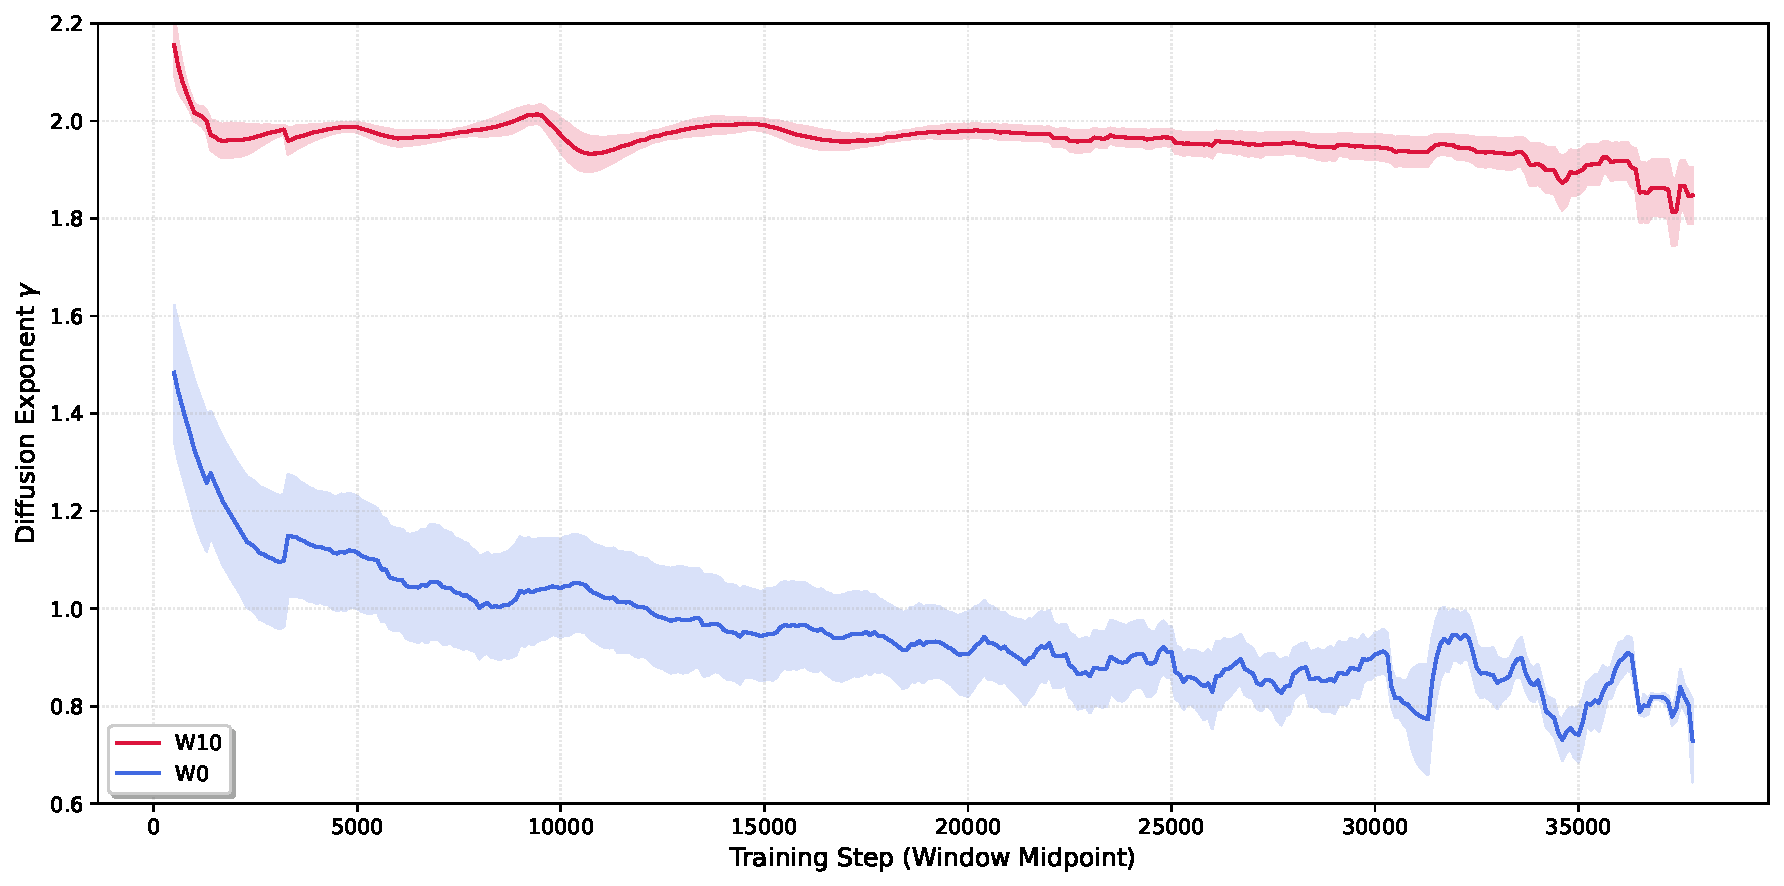
\includegraphics[width=0.8\textwidth]{diffusion_curve.pdf}
    \caption{Evolution of the diffusion exponent $\gamma$ for $W^{0}$ and $W^{10}$ over the training trajectory. Estimates are derived via a sliding window (width: 2000, stride: 200). Shaded regions represent the 95\% confidence interval ($1.96 \times \text{SE}$), acting as a proxy for the linearity and stability of the diffusion fit.}
    \label{fig:diffusion_curve}
\end{figure}
The decoupling of these regimes is tracked continuously in Figure \ref{fig:diffusion_curve}. The terminal layer maintains a robust near-ballistic state throughout training, evidenced by a tight confidence interval. In contrast, $W^{0}$ exhibits an initial super-diffusive burst before settling into a persistent sub-diffusive state. The swelling of the confidence interval for $W^{0}$ highlights the periods of maximum dynamical complexity, where the bend in the TAMSD profile is most pronounced. Near the limit of convergence (Steps 35,000+), we observe a mutual increase in fit instability, suggesting a transition toward a thermalised state for both layers as the global gradient signal dissipates.
\subsection{Structural Evolution and Spectral Re-Organisation}

% To characterise the morphological shifts occurring within the weight manifold during optimisation, we evaluate a suite of structural and spectral parameters derived from weight matrix snapshots. These metrics, presented in Figure \ref{fig:structure_metics}, quantify the transition from the initial random state to a learned functional configuration.

\begin{figure}[htbp]
	\centering
	\begin{subfigure}[b]{0.30\textwidth}
		\centering
		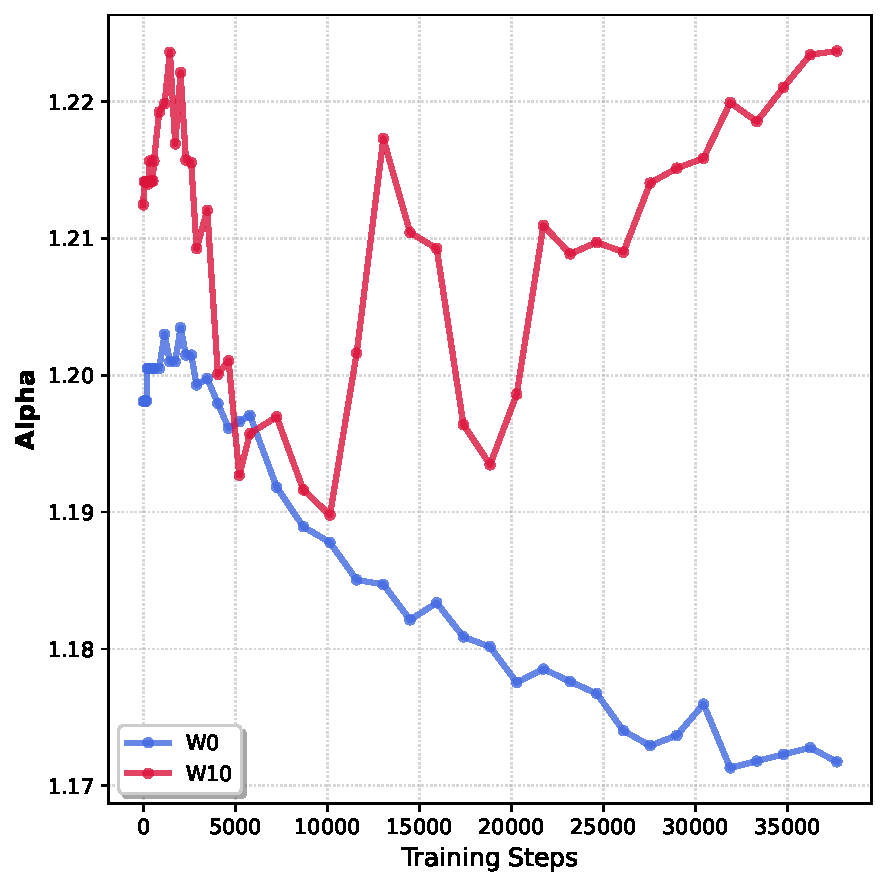
\includegraphics[width=\textwidth]{alpha_1.2_0.25.pdf}
		% \caption{Stability Parameter $\alpha$}
		\phantomcaption
		\label{fig:alpha}
	\end{subfigure}
	\begin{subfigure}[b]{0.30\textwidth}
		\centering
		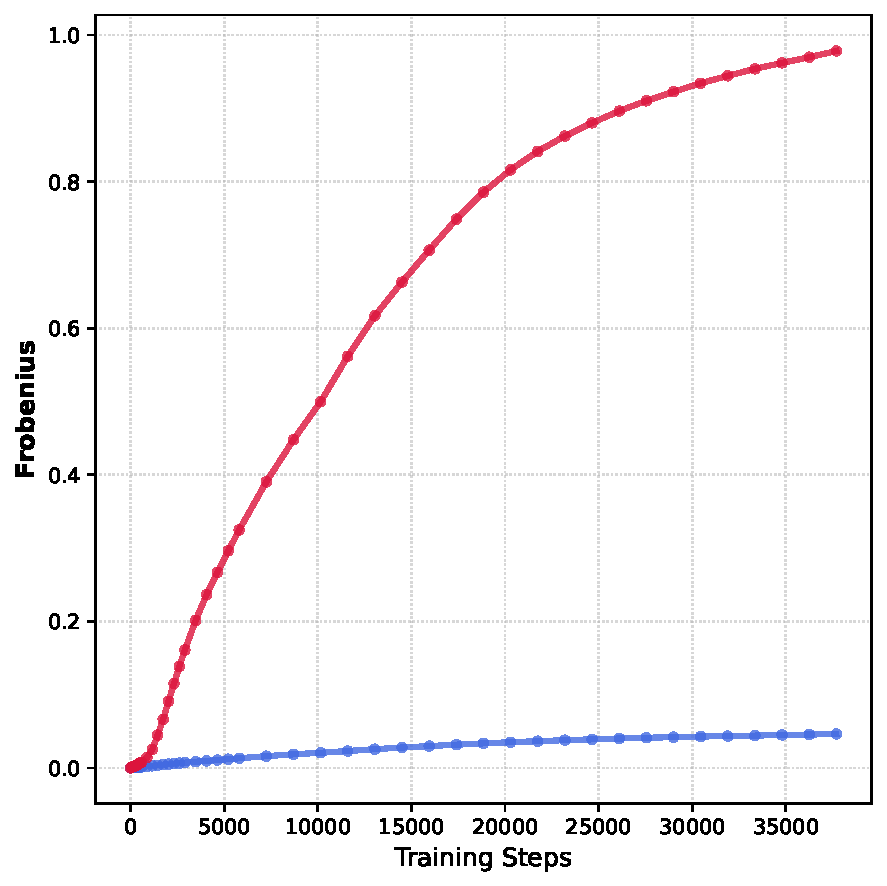
\includegraphics[width=\textwidth]{frobenius_1.2_0.25.pdf}
		% \caption{Rel. Frobenius Disp.}
		\phantomcaption
		\label{fig:frobenius}
	\end{subfigure}
	\begin{subfigure}[b]{0.30\textwidth}
		\centering
		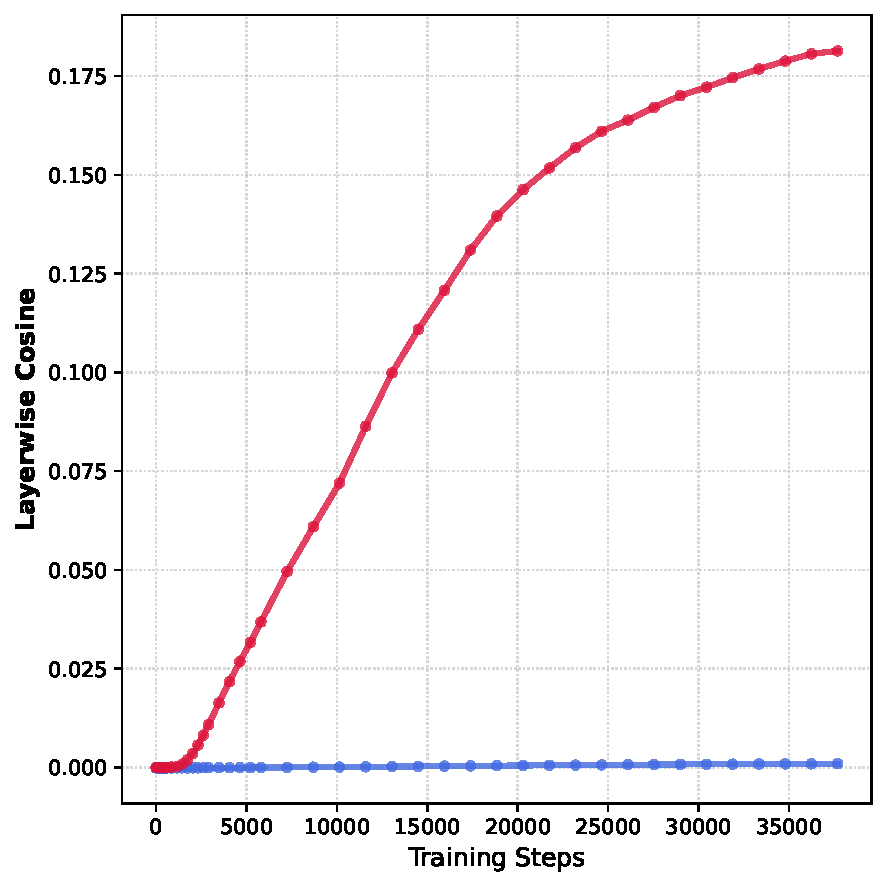
\includegraphics[width=\textwidth]{layerwise_cosine_1.2_0.25.pdf}
		% \caption{Cosine Distance}
		\phantomcaption
		\label{fig:cosine}
	\end{subfigure}
	\\[-2ex]
	\begin{subfigure}[b]{0.30\textwidth}
		\centering
		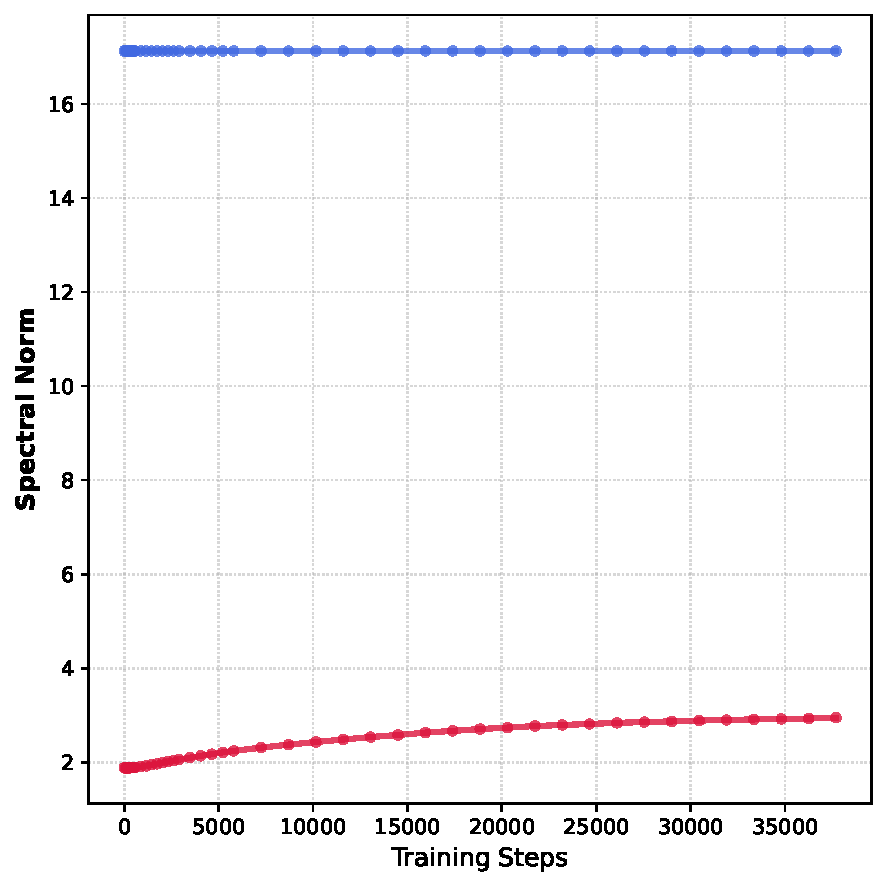
\includegraphics[width=\textwidth]{spectral_norm_1.2_0.25.pdf}
		% \caption{Spectral Norm $\|W\|_2$}
		\phantomcaption
		\label{fig:norm}
	\end{subfigure}
	\begin{subfigure}[b]{0.30\textwidth}
		\centering
		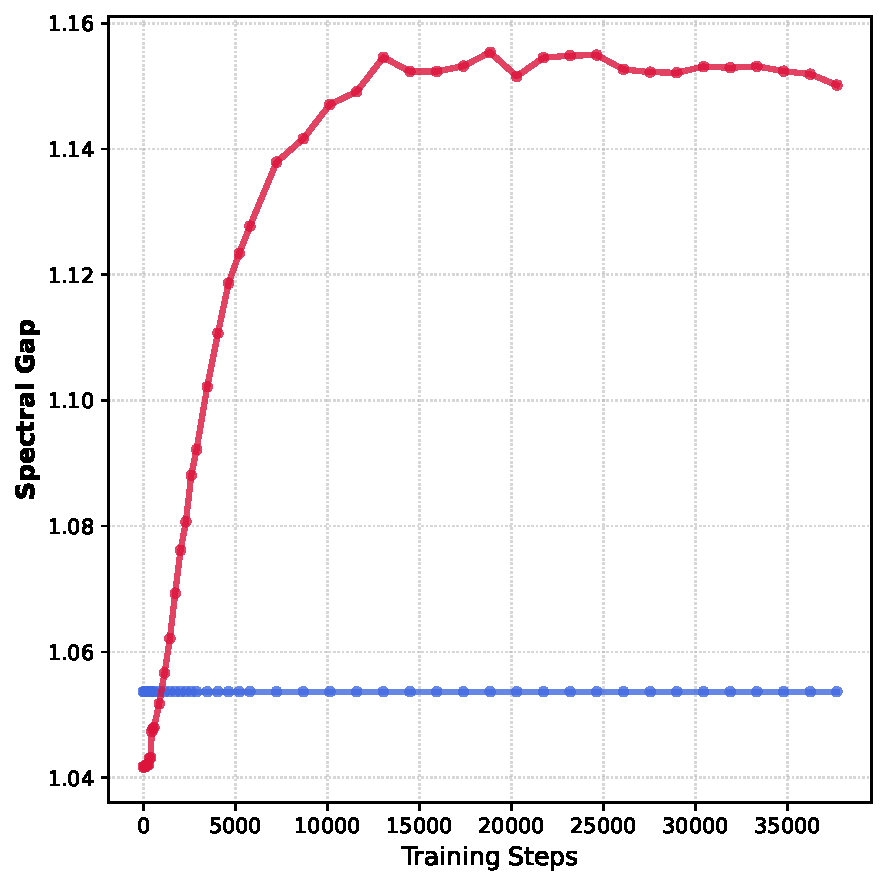
\includegraphics[width=\textwidth]{spectral_gap_1.2_0.25.pdf}
		% \caption{Spectral Gap}
		\phantomcaption
		\label{fig:gap}
	\end{subfigure}
	\begin{subfigure}[b]{0.30\textwidth}
		\centering
		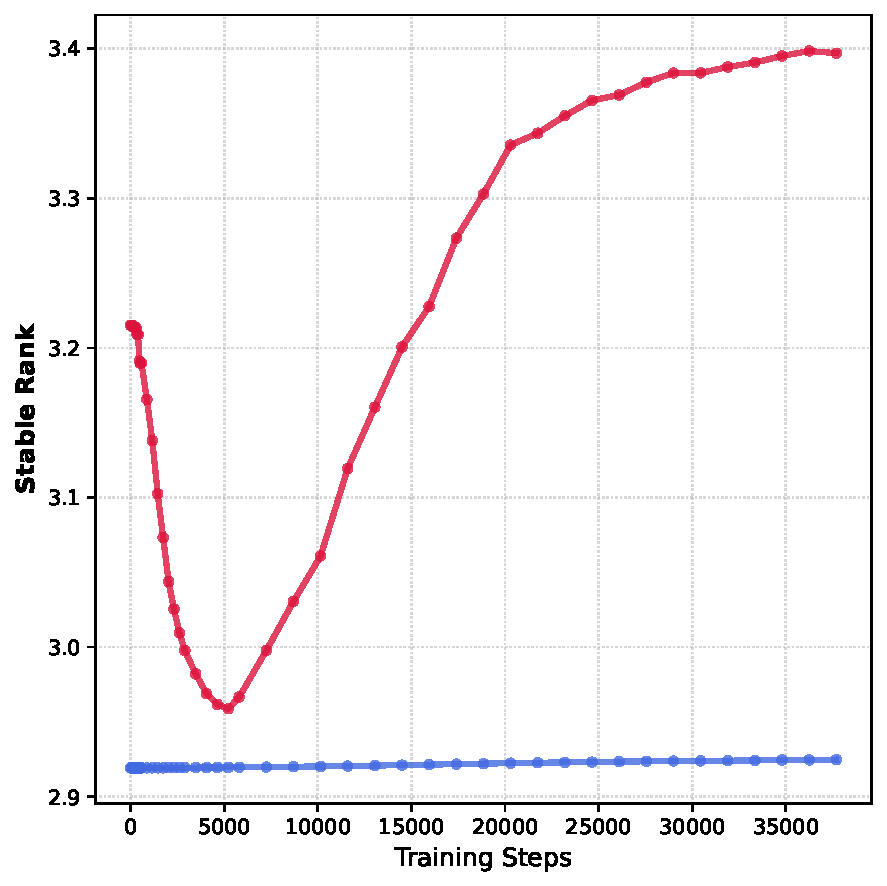
\includegraphics[width=\textwidth]{stable_rank_1.2_0.25.pdf}
		% \caption{Stable Rank}
		\phantomcaption
		\label{fig:rank}
	\end{subfigure}
	\vspace*{-2em}
	\caption{Structural and spectral evolution over training. (a) Heavy-tail stability parameter $\alpha$ via McCulloch estimation. (b) Relative Frobenius displacement $\|W_t - W_0\|_F / \|W_0\|_F$. (c) Layer-wise cosine distance $1 - (W_t \cdot W_0) / (\|W_t\|_F \|W_0\|_F)$. (d) Evolution of the spectral norm. (e) Spectral gap ($\lambda_1/\lambda_2$). (f) Stable rank $\|W\|_F^2 / \|W\|_2^2$, indicating effective dimensionality.}
	\label{fig:structure_metics}
\end{figure}

To characterise the morphological shifts occurring within the weight manifold during optimisation, we evaluate a suite of structural and spectral parameters derived from weight matrix snapshots. These metrics, presented in Figure \ref{fig:structure_metics}, quantify the transition from the initial random state to a learned functional configuration.

The structural metrics reveal a pronounced dynamical decoupling between the initial layer and the classifier. In Figure \ref{fig:alpha}, both $W^{0}$ and $W^{10}$ largely preserve the initial heavy-tail stability parameter $\alpha \approx 1.2$, though $W^{0}$ exhibits a slight relaxation toward $\alpha \approx 1.17$ by the terminal epoch. A stark divergence is observed in the Frobenius displacement (Fig. \ref{fig:frobenius}); for $W^{10}$, the relative displacement reaches $1.0$, indicating a global shift in weight magnitude equivalent to its initial norm. This correlates with the angular realignment shown in Figure \ref{fig:cosine}, where $W^{10}$ attains a cosine distance of $\approx 0.18$, representing a geometric rotation of approximately $35^\circ$ from the initialisation. In contrast, the input layer $W^{0}$ remains effectively stationary across both magnitude and orientation.

The spectral evolution further corroborates this specialisation. For $W^{10}$, we observe an increase in both the spectral norm (Fig. \ref{fig:norm}) and the spectral gap (Fig. \ref{fig:gap}, from $1.04$ to $1.15$), signalling the emergence of dominant singular vectors that characterise the learned features. The stable rank (Fig. \ref{fig:rank}) for $W^{10}$ exhibits a non-monotonic trajectory, dropping from $3.2$ to $2.95$ during the initial $5000$ steps, indicative of spectral compression—before rising toward $3.4$ as the weights stabilise. Throughout these spectral transformations, $W^{0}$ exhibits negligible deviation from its initial random state, suggesting a regime of lazy learning in the input features compared to the rich learning dynamics of the classifier.

\begin{figure}[htbp]
	\centering
	\begin{subfigure}{0.48\textwidth}
		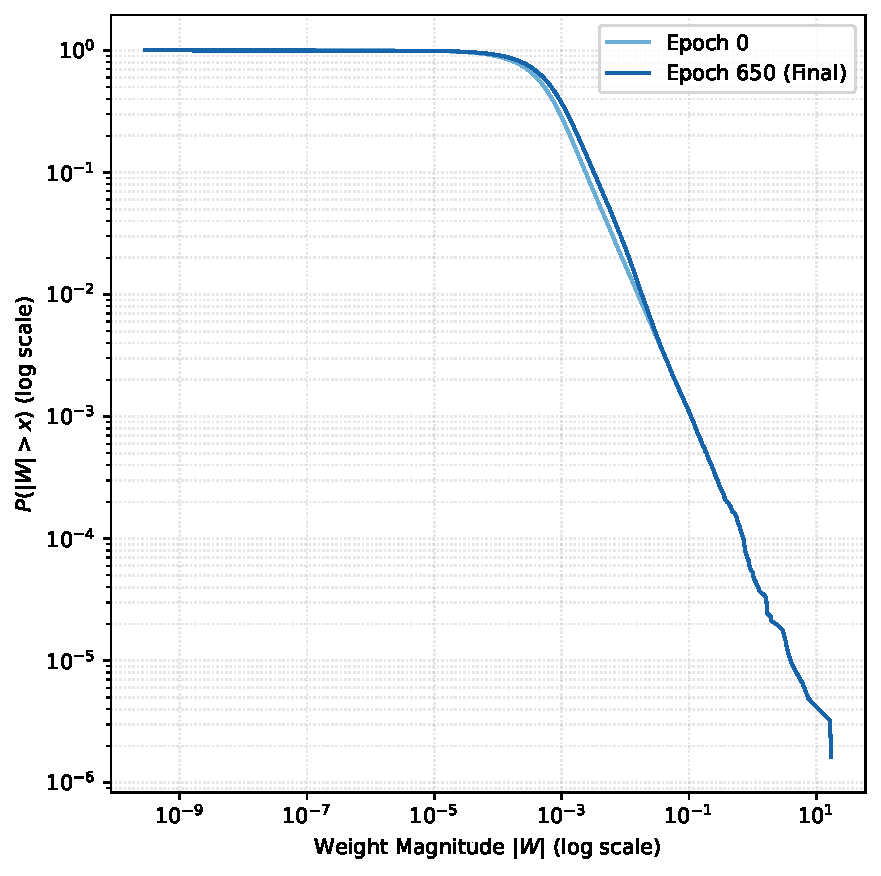
\includegraphics[width=\textwidth]{ccdf_initial.pdf}
		% \caption{CCDF Evolution: $W^{0}$}
		\phantomcaption
		\label{fig:ccdf_initial}
	\end{subfigure}
	\begin{subfigure}{0.48\textwidth}
		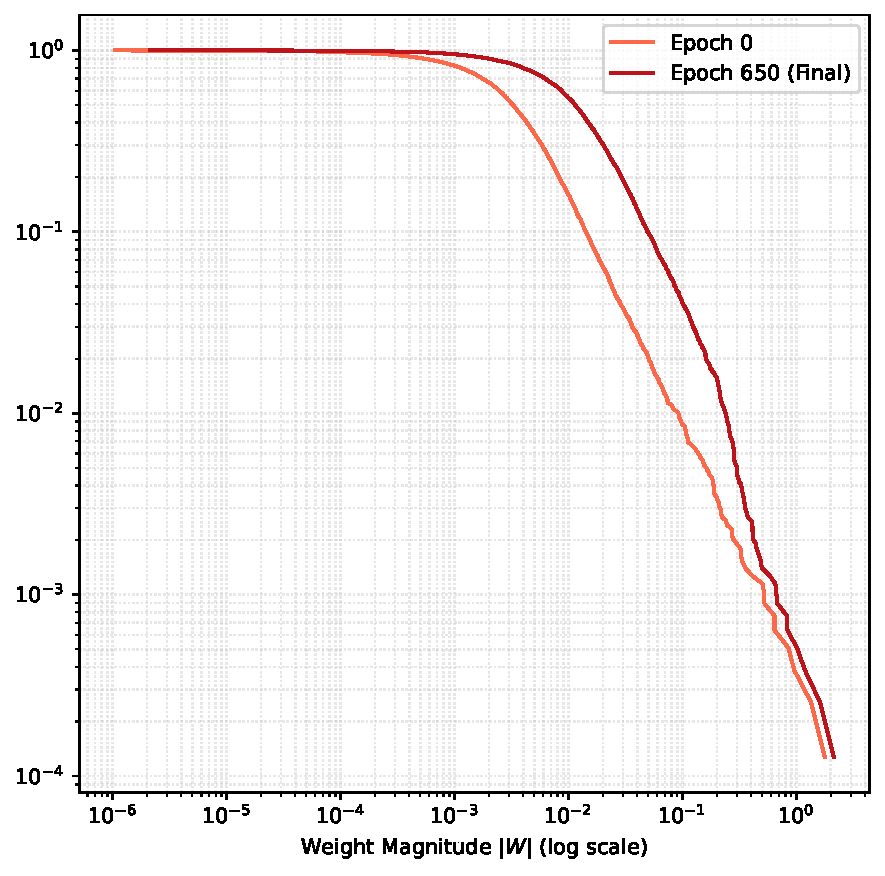
\includegraphics[width=\textwidth]{ccdf_classifier.pdf}
		% \caption{CCDF Evolution: $W^{10}$}
		\phantomcaption
		\label{fig:ccdf_classifier}
	\end{subfigure}
	\vspace*{-2em}
	\caption{Pre- and post-training Complementary Cumulative Distribution Functions (CCDF). (a) $W^{0}$ displays high distributional stability. (b) $W^{10}$ exhibits a significant rightward shift in the bulk and a steepening of the tail, suggesting structural regularisation.}
	\label{fig:ccdf}
\end{figure}

The structural transition is ultimately captured by the Complementary Cumulative Distribution Functions (CCDF) in Figure \ref{fig:ccdf}. While $W^{0}$ remains distributionally invariant (Fig. \ref{fig:ccdf_initial}), $W^{10}$ undergoes a significant global translation toward higher magnitudes (Fig. \ref{fig:ccdf_classifier}). Interestingly, we observe a concurrent steepening of the tail for weight magnitudes exceeding $2 \times 10^{-1}$, where the extreme outliers are suppressed relative to the shifted bulk. This behaviour suggests a dual mechanism of expansion and regularisation, where the network prunes extreme outliers during its ballistic ascent. Collectively, these structural signatures provide a microscopic basis for the macroscopic transport kinetics observed in the TAMSD analysis.
\newpage
\section{Discussion}
The results presented in this study provide a high-resolution window into the transport physics and structural reorganisation of neural networks initialised within the extended critical regime. By synthesising kinetic observables with spectral and distributional metrics, we identify a fundamental mechanism of \textit{Dynamical Phase Separation} that enables learning in regimes where standard Gaussian initialisation typically fail.

\subsection{Spatial Decoupling and the Hierarchical Division of Labour}

The most striking empirical finding is the emergence of a robust block-diagonal structure in the inter-layer correlation matrices (Fig. 3). This partitioning indicates that the network is not a monolithic dynamical entity but rather a decoupled system consisting of two functionally distinct regions:

\begin{itemize}
	\item \textbf{The Stochastic Reservoir ($W^1$--$W^7$):} These layers exhibit lazy learning characteristics, maintaining their initial heavy-tailed distribution ($\alpha \approx 1.2$) and geometric orientation throughout training. The anomalous sub-diffusive behaviour at short time lags ($\gamma \approx 0.78$) suggests these layers act as a stable, signal-preserving foundation that filters stochastic noise while resisting significant structural drift.
	\item \textbf{The Ballistic Classifier ($W^8$--$W^{10}$):} In contrast, the terminal layers operate in a high-energy, directed state. The near-perfect ballistic exponent ($\gamma \approx 1.97$) indicates that updates in this region are highly persistent and driven by a consistent gradient signal, performing the heavy lifting of functional specialisation.
\end{itemize}

This decoupling suggests that heavy-tailed initialisation facilitates a hierarchical division of labour: shallow layers provide the stability required for deep signal propagation, while deep layers leverage the infinite variance of the distribution to perform rapid structural realignments.

\subsection{The Geometry of Ballistic Realignment}

The nature of the classifier's movement provides a critical insight into the mechanics of rich learning. While the total $L_2$ displacement of $W^{10}$ is nearly an order of magnitude higher than $W^0$, we observe that its net drift (mean raw displacement) is significantly lower. This apparent paradox is resolved by the angular metrics: the classifier is not undergoing a simple translation in parameter space, but rather a geometric realignment.

The observed $35^\circ$ rotation in the weight vector indicates that $W^{10}$ is pivoting to align its weights with the dominant features emerging from the reservoir. This rotation is coupled with spectral condensation, as evidenced by the rising spectral gap and the initial drop in stable rank (Fig. 6). Collectively, these signatures indicate that the ballistic regime is defined by the compression of information into a low-rank manifold, allowing the network to lock onto a functional representation.

\subsection{Lévy Flights as a Mechanism for Minimum Escape}

The success of the $\alpha=1.2$ initialisation in the ordered regime ($\sigma=0.25$) is arguably the most compelling evidence for the advantages of extended criticality. In this regime, Gaussian networks exhibit stagnant accuracy, yet heavy-tailed networks demonstrate a staircase performance trajectory characterised by prolonged plateaus and abrupt bursts (Fig. 1).

We hypothesise that these bursts are driven by Lévy flights, discrete, high-magnitude realignments in the deep layers that allow the system to leap across energy barriers in the loss landscape. Where a Gaussian optimiser would remain trapped in a local minimum, the heavy-tailed weights leverage their infinite-variance tails to navigate to superior minima, driving the observed non-uniform learning behaviour.

\subsection{Stability through Expansion-Regularisation Duality}

A persistent question in the study of non-Gaussian initialisation is how the network maintains stability despite the risk of chaotic informational expansion. Our CCDF analysis suggests a dual mechanism: as the distribution expands to higher magnitudes (rightward shift), the tail simultaneously steepens (Fig. 7).

This suggests a form of structural self-regularisation or pruning, where the largest outliers are suppressed during the ballistic sprint. This duality prevents the system from diverging into chaos while still allowing it the energy required for directed realignment. This expansion-regularisation cycle appears to be a unique feature of the heavy-tailed training process, providing a microscopic basis for the stability of the extended critical regime.
\section{Conclusion}
\end{document}